\chapter{Recibir entrada del usuario}
   \label{Interaccion-Usuario}

\section{Interactuar con el teclado}
   \label{Interactuar-Teclado}
   \index{Teclado}

Durante la ejecuci\'on del programa, se puede recibir texto ingresado
por el usuario a trav\'es de 3 primitivas:
\texttt{tecla?}, \index{tecla?@\texttt{tecla?}}
\texttt{leecar} \index{leecar@\texttt{leecar}} y
\texttt{leelista}. \index{leelista@\texttt{leelista}}
\begin{itemize}
   \item \texttt{tecla?}: Da \texttt{cierto} o \texttt{falso} seg\'un se haya
      pulsado o no alguna tecla desde que se inici\'o la ejecuci\'on del
      programa. 
   \item \texttt{leecar} o \texttt{leetecla}:
      \index{leetecla@\texttt{leetecla}}
      \begin{itemize}
         \item Si \texttt{tecla?} es \texttt{falso}, el programa hace una
            pausa hasta que el usuario pulse alguna tecla.
         \item Si \texttt{tecla?} es \texttt{cierto}, da la \'ultima tecla
            que haya sido pulsada.
      \end{itemize}
      Estos son los valores que dan ciertas teclas:
      \begin{center}\begin{tabular}{|c|c|c|c|c|} \hline 
         A  $\rightarrow$  65 & B  $\rightarrow$  66 & C  $\rightarrow$  67 & \ldots
            & Z  $\rightarrow$  90 \\ \hline
         $\triangleleft$ $\rightarrow$ -37 \'o -226 &
           $\bigtriangleup$ $\rightarrow$ -38 \'o -224 &
              $\triangleright$ $\rightarrow$ -39 \'o -227 &
                 $\bigtriangledown$ $\rightarrow$ -40 \'o -225 & \\ \hline 
         \texttt{Esc} $\rightarrow$  27 & \texttt{F1}  $\rightarrow$  -112 &
           \texttt{F2}  $\rightarrow$  -113 & \ldots &
             \texttt{F12}  $\rightarrow$  -123 \\ \hline
         \texttt{SHIFT}  $\rightarrow$  -16 & \texttt{ESPACIO}  $\rightarrow$  32 &
           \texttt{CTRL}  $\rightarrow$  -17 & \texttt{ENTER}  $\rightarrow$  10 & \\
              \hline
      \end{tabular} \end{center}
      Si tienes dudas acerca del valor que da alguna tecla, puedes probar
      con: \texttt{es leecar}. El int\'erprete esperar\'a hasta que
      pulses una tecla, y escribir\'a su valor.
   \item \texttt{leelista [t\'itulo] \char`\"palabra} o%
      \index{leeteclado@\texttt{leeteclado}}
      \texttt{leeteclado [t\'itulo] \char`\"{}palabra}: Presenta una caja de
      di\'alogo titulada \texttt{t\'itulo}. El usuario puede escribir
      un texto en el \'area de entrada, y esta respuesta se guardar\'a
      seleccionando autom\'aticamente si en forma de n\'umero o de lista
      en la variable \texttt{:palabra} cuando se haga \textit{click} en el
      bot\'on \texttt{OK}.
\end{itemize}

Las primitivas \texttt{caracter}, \index{caracter@\texttt{caracter}}(su forma 
corta es \texttt{car} \index{car@\texttt{car}}y cuyo argumento es \texttt{n}: un n\'umero) y \texttt{unicode} \verb+"a+,\index{unicode@\texttt{unicode}} devuelven,
respectivamente, el car\'acter unicode que corresponde al n\'umero \texttt{n}
y el n\'umero unicode que corresponde al car\'acter \texttt{a}. \\

\textbf{Ejemplo}: \begin{verbatim}
    unicode "A            devuelve      65
    caracter 125          devuelve      } \end{verbatim}

\begin{quote}
   \noindent \textbf{Ejemplos}:
   \begin{quote}
      \verb+para edades+\\
      \verb+  leelista +\texttt{[?`Qu\'e edad tienes?] \char`\"{}edad}\\
      \verb+  si :edad < 18 [escribe [Eres menor]]+\\
      \verb+  si :edad > 17 [escribe [Eres adulto]]+\\
      \verb+  si :edad > 69 [escribe [Con todo respeto!!]]+\\
      \verb+fin+\\

      \verb+para dibujar+ \\
      \verb+# La tortuga es controlada con las flechas del teclado.+ \\
      \verb+# Se termina con Esc.+ \\
      \verb+si tecla?+ \\
      \verb+  [ haz "valor leecar+ \\
      \verb+    si :valor=-37 [giraizquierda 90]+ \\
      \verb+    si :valor=-39 [giraderecha 90]+ \\
      \verb+    si :valor=-38 [avanza 10]+ \\
      \verb+    si :valor=-40 [retrocede 10]+ \\
      \verb+    si :valor=27 [alto] ]+ \\
      \verb+ dibujar+ \\
      \verb+fin+\end{quote}
\end{quote}

\section{Interactuar con el rat\'on}
    \label{Interactuar-Raton}
    \index{Rat\'on}

Durante la ejecuci\'on del programa, se pueden recibir eventos del rat\'on
a trav\'es de tres primitivas:
\texttt{leerat\'on}, \index{leerat\'on@\texttt{leerat\'on}}
\texttt{rat\'on?} \index{rat\'on?@\texttt{rat\'on?}} y
\texttt{posrat\'on}.\index{posrat\'on@\texttt{posrat\'on}}

\begin{itemize}
   \item \texttt{leerat\'on}: el programa espera hasta que el usuario hace
      un \textit{click} o un movimiento. Entonces, devuelve un n\'umero que
      representa ese evento. Los posibles valores son:
      \begin{itemize}
         \item 0 $\rightarrow$ El rat\'on se movi\'o.
         \item 1 $\rightarrow$ Se hizo un \textit{click} izquierdo.
         \item 2 $\rightarrow$ Se hizo un \textit{click} central (se usa en Linux).
         \item 3 $\rightarrow$ Se hizo un \textit{click} derecho.
      \end{itemize}
   \item \texttt{posrat\'on}: Da una lista que contiene la posici\'on actual del
      rat\'on.
   \item \texttt{rat\'on?}: Devuelve \texttt{cierto} o \texttt{falso} seg\'un
      toquemos o no el rat\'on desde que comienza la ejecuci\'on del programa
\end{itemize}


\noindent \textbf{Ejemplos}:

En este primer procedimiento, la tortuga sigue los movimientos del rat\'on por
la pantalla. \\

\noindent \texttt{para seguir}

\noindent \texttt{\# cuando el rat\'on se mueve, la tortuga cambia de posici\'on}

 \texttt{ si leerat\'on=0 [ponposici\'on posrat\'on]}

 \texttt{ seguir}

\noindent \texttt{fin} \\

\noindent Este segundo procedimiento es similar, pero hay que hacer \textit{click}
izquierdo para que la tortuga se mueva.: \\

\noindent \texttt{para seguir2}

\texttt{si leerat\'on = 1 [ponposici\'on posrat\'on]}

\texttt{seguir2}

\noindent \texttt{fin} \\

\noindent En este tercer ejemplo, hemos creado dos botones rosa. Si hacemos
   \textit{click} izquierdo, la tortuga dibuja un cuadrado de lado 40. Si
   hacemos \textit{click} derecho, la tortuga dibuja un peque\~no c\'irculo.
   Por \'ultimo si hacemos \textit{click} derecho en el bot\'on derecho, se
   detiene el programa.

   \begin{center}
      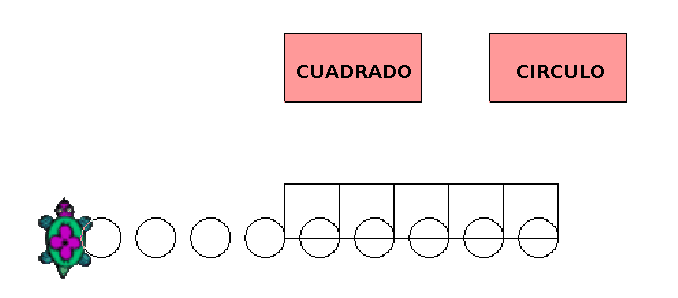
\includegraphics[scale=0.6]{Imagenes/10_Usuario/CtrlRaton.png}
   \end{center}

\noindent \texttt{para bot\'on}

\noindent \texttt{\# crea un bot\'on rectangular color rosa, de 50 x 100}

\texttt{repite 2 [}

\texttt{avanza 50 giraderecha 90 avanza 100 giraderecha 90 ]}

\texttt{giraderecha 45 subelapiz avanza 10}

\texttt{bajal\'apiz poncolorl\'apiz [255 153 153]}

\texttt{rellena retrocede 10 giraizquierda 45 bajal\'apiz poncolorl\'apiz 0}

\noindent \texttt{fin} \\

\noindent \texttt{para empieza}

\texttt{borrapantalla bot\'on subel\'apiz ponposici\'on [150 0]}

\texttt{bajal\'apiz bot\'on subel\'apiz ponposici\'on [30 20] bajal\'apiz}

\texttt{rotula \char`\"{}Cuadrado subel\'apiz ponposici\'on [180 20]}

\texttt{bajal\'apiz rotula "C\'irculo}

\texttt{subel\'apiz ponposici\'on [0 -100] bajal\'apiz}

\texttt{rat\'on}

\noindent \texttt{fin} \\

\noindent \texttt{para rat\'on}

\noindent \texttt{\# ponemos el valor de leerat\'on en la variable ev}

\noindent \texttt{\# ponemos la primera coordenada en la variable x}

\noindent \texttt{\# ponemos la segunda coordenada en la variable y}

\texttt{haz \char`\"{}ev leerat\'on}

\texttt{haz \char`\"{}x elemento 1 posrat\'on}

\texttt{haz \char`\"{}y elemento 2 posrat\'on}

\noindent \texttt{\# si hay click izquierdo}

\texttt{si :ev=1 \& :x>0 \& :x<100 \& :y>0 \& :y<50 [cuadrado]}

\noindent \texttt{\# si hay click derecho}

\texttt{si :x>150 \& :x<250 \& :y>0 \& :y<50 [}

\texttt{si :ev=1 [circunferencia]}

\texttt{si :ev=3 [alto] ]}

\texttt{rat\'on}

\noindent \texttt{fin} \\

\noindent \texttt{para circunferencia}

\texttt{repite 90 [avanza 1 giraizquierda 4]}

\texttt{giraizquierda 90 subel\'apiz avanza 40 giraderecha 90 bajal\'apiz}

\noindent \texttt{fin} \\

\noindent \texttt{para cuadrado}

\texttt{repite 4 [avanza 40 giraderecha 90]}

\texttt{giraderecha 90 avanza 40 giraizquierda 90}

\noindent \texttt{fin}

\section{Componentes Gr\'aficos}

Desde la versi\'on 0.9.90, XLogo permite a\~nadir componentes gr\'aficos en el
\'Area de dibujo (botones, men\'us, \ldots) \\

Las primitivas que permiten crear y modificar estos componentes terminan con el
sufijo \texttt{igu} (Interfaz Gr\'afica de Usuario -- \textit{Graphical User
Interface, gui} son sus siglas inglesas).

\subsection{Crear un componente gr\'afico}

La secuencia de pasos que debes seguir es: \textbf{Crear}  $\rightarrow$ 
\textbf{Modificar} sus propiedades o caracter\'isticas  $\rightarrow$  \textbf{Mostrar}lo
en el \'Area de dibujo.

\subsubsection{Crear un Bot\'on}

Usaremos al primitiva \texttt{botonigu}, \index{botonigu@\texttt{botonigu}}cuya
sintaxis es: 

\noindent \texttt{\# Esta primitiva crea un bot\'on llamado b}

\noindent \texttt{\# y cuya leyenda es: Click}

\noindent \texttt{botonigu \char`\"{}b \char`\"{}Click}

\subsubsection{Crear un Men\'u}

Disponemos de la primitiva \texttt{menuigu}, 
\index{menuigu@\texttt{menuigu}}cuya sintaxis es:

\noindent \texttt{\# Esta primitiva crea un men\'u llamado m}

\noindent \texttt{\# y que contiene 3 opciones: opci\'on1, opci\'on2 y opci\'on3}

\noindent \texttt{menuigu \char`\"{}m [opci\'on1 opci\'on2 opci\'on3]}

\subsubsection{Modificar las propiedades del componente gr\'afico}

\texttt{posicionigu} \index{posicionigu@\texttt{posicionigu}}
determina las coordenadas donde se colocar\'a el elemento gr\'afico.
Por ejemplo, para colocar el bot\'on definido antes en el punto de coordenadas 
\texttt{(20 , 100)}, escribiremos:
\begin{verbatim}
posicionigu "b [20 100] \end{verbatim}

Si no se especifica la posici\'on, el objeto ser\'a colocado por defecto en la
esquina superior izquierda del \'Area de dibujo.

\subsubsection{Eliminar un componente gr\'afico}

La primitiva \texttt{eliminaigu} \index{eliminaigu@\texttt{eliminaigu}}
elimina un componente gr\'afico. Para eliminar el bot\'on anterior
\begin{verbatim}
eliminaigu "b \end{verbatim}

\subsubsection{Definir acciones asociadas a un componente gr\'afico}

La primitiva \texttt{accionigu}, \index{accionigu@\texttt{accionigu}}
define una acci\'on asociada al componente, y que se realizar\'a cuando el
usuario interact\'ua con \'el. \\

\noindent \texttt{\# Que la tortuga avance 100 al pulsar el boton \char`\"{}b}

\noindent \texttt{accionigu \char`\"{}b [avanza 100 ]}

\noindent \texttt{\# En el men\'u, cada opci\'on indica su acci\'on}

\noindent \texttt{accionigu \char`\"{}m [[escribe \char`\"{}Opci\'on1]
  [escribe \char`\"{}Opci\'on2] [escribe \char`\"{}Opci\'on3]]} 

\subsubsection{Dibujar el componente gr\'afico}

La primitiva \texttt{dibujaigu}, \index{dibujaigu@\texttt{dibujaigu}}
muestra el componente gr\'afico en el \'Area de dibujo. Para mostrar el
bot\'on que estamos usando como ejemplo:
\begin{verbatim}
dibujaigu "b \end{verbatim}
\begin{center}
   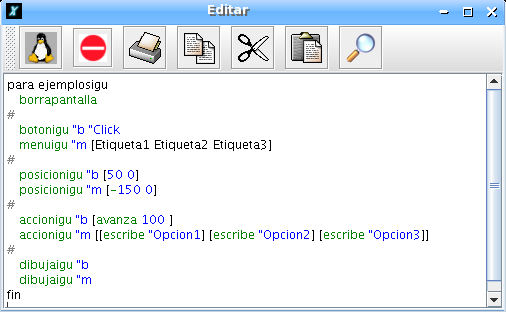
\includegraphics[scale=0.45]{Imagenes/10_Usuario/EjemplosIGU_01.png} \hfill
   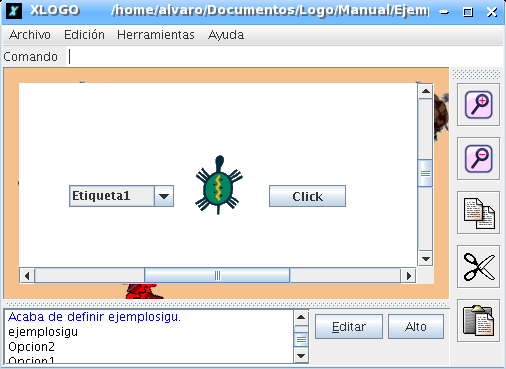
\includegraphics[scale=0.4]{Imagenes/10_Usuario/EjemplosIGU_02.png} 
\end{center}

Corrijamos el ejemplo anterior utilizando las nuevas primitivas:

\noindent \texttt{para empieza}

\texttt{botonigu \char`\"{}Boton.Circ \char`\"{}C\'irculo}

\texttt{botonigu \char`\"{}Boton.Cuad \char`\"{}Cuadrado}

\texttt{posicionigu \char`\"{}Boton.Circ   [50 100]}

\texttt{posicionigu \char`\"{}Boton.Cuad [-150 100]}

\texttt{accionigu \char`\"{}Boton.Circ [ circunferencia ]}

\texttt{accionigu \char`\"{}Boton.Cuad [ cuadrados ]}

\texttt{dibujaigu \char`\"{}Boton.Circ}

\texttt{dibujaigu \char`\"{}Boton.Cuad}

\noindent \texttt{fin} \\

\noindent \texttt{para circunferencia}

\texttt{repite 90 [av 1 gi 4]}

\texttt{giraizquierda 90 subel\'apiz avanza 40 giraderecha 90 bajal\'apiz}

\noindent \texttt{fin} \\

\noindent \texttt{para cuadrado}

\texttt{repite 4 [avanza 40 giraderecha 90]}

\texttt{giraderecha 90 avanza 40 giraizquierda 90}

\noindent \texttt{fin}
\begin{center}
   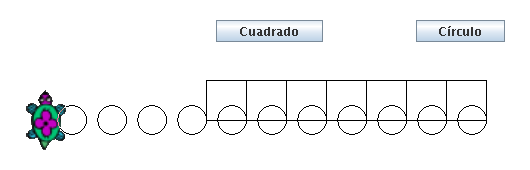
\includegraphics[scale=0.8]{Imagenes/10_Usuario/EjemplosIGU_03.png}
\end{center}